\documentclass{izpit}

\begin{document}

%==========================================================================
%               Sem vpisi podatke o izpitu
%==========================================================================
\FRACTIONSIMPLIFY{60}{1}{\skupnotock}{\nepomembno}%Sem vpiši (v polje trenutno {60}) skupno število točk, da paket naračuna kriterij ocenjevanj
\izpit[ucilnica = ROSKA, naloge = 3]%ucilnica ROSKA ali KRIZANKE, lahko se sedezni red, ime in priimek, maturitetni
{Matematika - Polinomi}{30. 9. 2239}{Čas pisanja je 45 minut.\\ Možno je doseči $\skupnotock$ točk.\\ Veliko uspeha!}
%==========================================================================
%               Nepomembno - Preskoči
%==========================================================================
\MAX{0.1}{0}{\tempepsilon}%shranimo epsilon... ne gre trik z ulomkom zato max
\MULTIPLY{\skupnotock}{0.9}{\odlicno}
\MULTIPLY{\skupnotock}{0.76}{\pravdobro}
\MULTIPLY{\skupnotock}{0.63}{\dobro}
\MULTIPLY{\skupnotock}{0.5}{\zadostno}
\ADD{\dobro}{\tempepsilon}{\dobroplus}
\ADD{\pravdobro}{\tempepsilon}{\pravdobroplus}
\ADD{\odlicno}{\tempepsilon}{\odlicnoplus}
\ROUND[1]{\dobroplus}{\dobroplus}
\ROUND[1]{\pravdobroplus}{\pravdobroplus}
\ROUND[1]{\odlicnoplus}{\odlicnoplus}
\ROUND[1]{\zadostno}{\zadostno}
\ROUND[1]{\dobro}{\dobro}
\ROUND[1]{\pravdobro}{\pravdobro}
\ROUND[1]{\odlicno}{\odlicno}\begin{small}
 \PlaceText{100mm}{33mm}{\begin{tabular}{ll}
    \multicolumn{2}{c}{\textbf{Kriterij ocenjevanja}} \\[0.5ex]
    Ocena & Tocke \\ \hline
    zadostno & $\zadostno - \dobro$ \\
    dobro & $\dobroplus - \pravdobro$ \\
    prav dobro & $\pravdobroplus - \odlicno$ \\
    odlicno & $\odlicnoplus$--
  \end{tabular}}\end{small}
 \ifthenelse{\boolean{@maturitetni}}{\newpage}%TO JE ZELO GRDA KODA a ker ne gre kriterij v class ni druge moznosti
%==========================================================================
%               Sem vpisi naloge
%   za dodatek koordinatnega sistema daj pod navodila naloge \dodatek{\[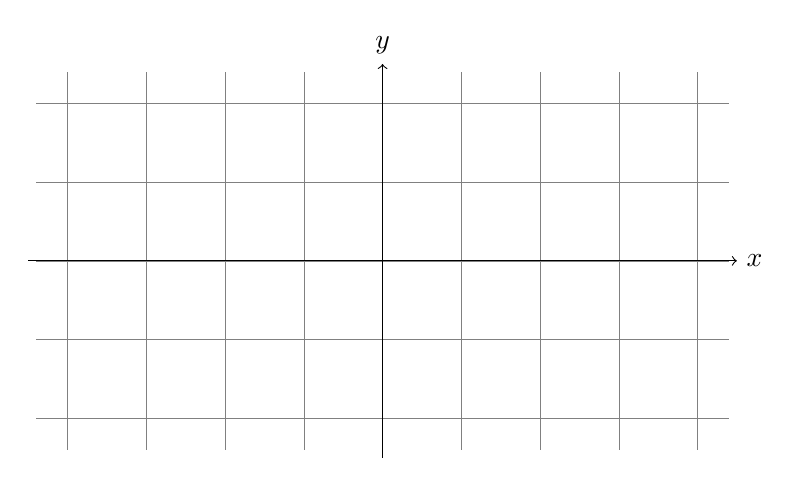
\begin{tikzpicture}
        \draw[help lines,step=1cm] (-4.4,-2.4) grid (4.4,2.4);
        \draw[->] (-4.5,0) -- (4.5,0) node[right] {$x$};
        \draw[->] (0,-2.5) -- (0,2.5) node[above] {$y$};
\end{tikzpicture}\]}
%   oz. za kompleksno ravnino \dodatek\[\begin{tikzpicture}
        \draw[help lines,step=1cm] (-4.4,-2.4) grid (4.4,2.4);
        \draw[->] (-4.5,0) -- (4.5,0) node[right] {$Re$};
        \draw[->] (0,-2.5) -- (0,2.5) node[above] {$Im$};
\end{tikzpicture}\]
%==========================================================================

\naloga[\tocke{16}]
  Skicirajte graf funkcije $f \colon \mathbb{R} \to \mathbb{R}$, podane s
  predpisom
  \[
    f(x) = \frac{1 + x - x^2}{3 x^2 - 5} \;.
  \]

  % Ukaz \dodatek uporabite, kadar na izpit želite dati sliko, tabelo, ali kaj
  % podobnega, kar bo študentom v pomoč pri pisanju odgovorov.
  % Če paket naložite z možnostjo 'arhiv', ukaz \dodatek ne naredi ničesar.
  \dodatek{\[\begin{tikzpicture}
        \draw[help lines,step=1cm] (-4.4,-2.4) grid (4.4,2.4);
        \draw[->] (-4.5,0) -- (4.5,0) node[right] {$Re$};
        \draw[->] (0,-2.5) -- (0,2.5) node[above] {$Im$};
\end{tikzpicture}\]}
  
  
\naloga[\tocke{20}]
  \podnaloga[15]
  
  Poišči predpise spodnjih funkcij.
  \[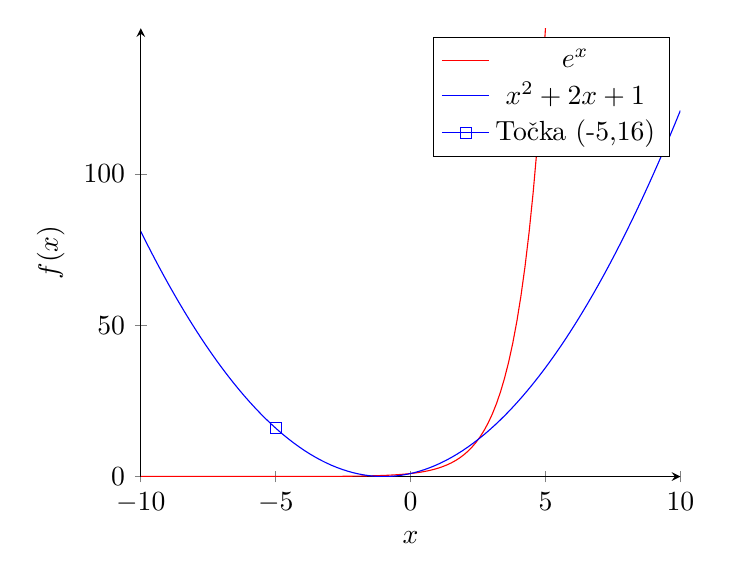
\begin{tikzpicture}

\begin{axis}[axis lines = left,xlabel = \(x\),ylabel = {\(f(x)\)}]%nastavimo parametri kakšen bo sam koordinatni sistem

%Eksponentna funkcija
\addplot [domain=-10:5, samples=100, color=red]{e^x};%domena
\addlegendentry{\(e^x\)} %doda opis funkcij


%Parabola
\addplot [domain=-10:10, samples=100, color=blue]{x^2 + 2*x + 1};
\addlegendentry{\(x^2 + 2x + 1\)}
%dodamo točke na paraboli
\addplot[color=blue, mark=square] coordinates {(-5,16)};\addlegendentry{Točka {(-5,16)}}
    
%Parabola
%\addplot[domain=0:2*pi]{sin(deg(x)}


\end{axis}
\end{tikzpicture}\]% ne damo v dodatek, saj hočemo prikaz v arhivu
    
  % Ukaz \prostor na polo doda prostor za rešitev. Ukaz sprejme neobvezen
  % argument, ki pove, kolikšen delež prostora naj bo namenjen nalogi.
  % Če paket naložite z možnostjo 'arhiv', ukaz \prostor ne naredi ničesar.
  \prostor[2] % Za to nalogo bo dvakrat toliko prostora kot za naslednjo.

  \podnaloga[5]
    Poiščite izjavo $X = X(p, q, r)$, ki ima naslednjo pravilnostno tabelo.
    Izjavo poenostavite do oblike, ki vsebuje kvečjemu dva logična veznika.
    \[
      \begin{tabular}{c|cccccccc}
        $p$ & 1 & 1 & 1 & 1 & 0 & 0 & 0 & 0 \\
        $q$ & 1 & 1 & 0 & 0 & 1 & 1 & 0 & 0 \\
        $r$ & 1 & 0 & 1 & 0 & 1 & 0 & 1 & 0 \\\hline
        $X$ & 1 & 0 & 1 & 0 & 1 & 0 & 1 & 1 \\
      \end{tabular}
    \]
  \prostor

% Vsaka naslednja naloga gre v osnovi na novo stran. Če želite nalogo dodati
% na isto stran, uporabite ukaz \naloga*, ki se obnaša enako kot \naloga, le
% da ne naredi nove strani.
\naloga*[dodatnih 5 točk]%se ne steje v procente za ocene

  Za katera cela števila $c$ ima diofantska enačba
  \[
    72 x + 19 y = c
  \]
  rešitve v celih številih? Kakšna je v tem primeru splošna oblika rešitve?

\end{document}